\documentclass{article}
\usepackage{graphicx}
\graphicspath{{Images/}}
\usepackage{hyperref}
\usepackage{adjustbox}
\usepackage{blindtext}
\usepackage{enumitem}
\usepackage{float}
\usepackage{array}
\begin{document} 
\title{\textbf{{\Huge PowerEnJoy project: Integration Test Plan Document}}}
\author{\begin{large}
Boriero Stefano  876106  
Brunitti Simone   875039
\end{large} }


\maketitle

\includegraphics[scale=0.5]{Images/Logo_Politecnico_Milano.png}
\newpage
\tableofcontents

\newpage
\section{Introduction}

\subsection{Revision History}
\subsection{Purpose and Scope}

The purpose of this ITPD (Integration Test Plan Document) is to describe how we intend to accomplish the integration testing of our PowerEnJoy platform. The components to be integrated are those identified in the DesignDocument that has been already written.

\subsection{List of Definitions and	Abbreviation}
\begin{itemize}
\item System: the whole PowerEnJoy system
\item Subsystem: a part of the system
\item Module: a part of a subsystem
\item Component: an atomic part of a module
\end{itemize}

\subsection{List of Reference Documents}
\begin{itemize}
\item \href{https://github.com/StefanoBoriero/PowerEnjoy_Boriero_Brunitti/blob/master/Assignments%20AA%202016-2017.pdf}{Assignment}
\item \href{https://github.com/StefanoBoriero/PowerEnjoy_Boriero_Brunitti/blob/master/releases/RASD_v1.md}{RASD}
\item \href{https://github.com/StefanoBoriero/PowerEnjoy_Boriero_Brunitti/blob/master/releases/DD%20v1.pdf}{Desing Document}
\item \href{https://developer.apple.com/library/content/documentation/Performance/Conceptual/PerformanceOverview/PerformanceTools/PerformanceTools.html}{iOS Test Tools}

\item \href{ https://msdn.microsoft.com/it-it/library/windows/apps/hh202934(v=vs.105).aspx}{Windows Phone Test Tools}
\item \href{https://developer.android.com/studio/profile/android-monitor.html}{Android Test Tools}
\end{itemize}

\newpage
\section{Integration Strategy}

\subsection{Entry Criteria}
Before starting the integration phase, we have to meet certain constraints on different aspects of the project.
\\\\
All components must have been unit tested
The integration procedure should start after these percentages of completion are reached:
\begin{itemize}
\item \textbf{100\%} of DatabaseController functionalities
\item At least \textbf{90\%} of Customer subsystem
\item At least \textbf{80\%} of Car subsystem
\item At least \textbf{50\%} of Employee subsystem
\end{itemize}

\subsection{Elements to be Integrated}
As it can be seen from the Design Document, the whole system can be divided into three major subsystem:
\begin{itemize}
\item \textbf{Customer subsystem}, offering functionalities to exploit the services provided by the car sharing company

\item \textbf{Employee subsystem}, offering functionalities for company's employee to manage the system

\item \textbf{Car subsystem}, offering functionalities to dialog with cars
\end{itemize}

Each of this subsystems is divided into submodules encapsulating the components related to a group of functionalities in this way:
\begin{itemize}
\item \textbf{Customer subsystem}:
\begin{itemize}
\item \textit{ReservationController}: offers the user functionalities to manage a reservation
\item \textit{BalanceController}: offers the user functionalities to manage his balance
\item \textit{AccountController}: offers the user functionalities to manage his account
\item \textit{RegistrationController}: offers the user functionalities to register to the system
\item \textit{ReportController}: offers the user functionalities to notify issues
\end{itemize}
\item \textbf{Employee subsystem}:
\begin{itemize}
\item \textit{SafeAreaController}: offers the employee functionalities to manage safe areas
\item \textit{AssistanceController}: offers the employee functionalities to manage needy cars
\end{itemize}
\item \textbf{Car subsystem}:
\begin{itemize}
\item \textit{CarController}: offers the system functionalities to send commands to the car
\item \textit{RideController}: offers the CarApp the functionalities to manage a ride
\item \textit{BillController}: offers functionalities to calculate bills
\item \textit{FaultController}: offers the CarApp the functionalities to manage faults
\item \textit{FleetController}: offer the CarApp the functionalities to join and detach from the fleet
\end{itemize}
\end{itemize}


The elements to be integrated are the components of these submodules

\subsection{Integration Testing Strategy}
We will follow a functional grouping approach, grouping components in the submodules presented above. We will first integrate functional groups of Employee subsystem, as these exploited also by the other subsystems. Then we will proceed integrating functional groups of Car subsystem and Customer subsystem.
\\

For each functional group we will follow a bottom-up approach, and once integrated all submodules of a subsystem, we will integrate the subsystem with its dispatcher and web application. This will allow us to focus initially on binary integrations and to start testing complete functionalities as we proceed.

\subsection{Sequence of Component/Function Integration}

\subsubsection{Software Integration Sequence}

\begin{Large}
\textbf{Employee System Strategy}
\end{Large}

For testing the Employee System, we will use a bottom-up strategy. These are the separate modules we are going to test: 
\begin{enumerate}
\item SafeAreaController
\item AssistanceController
\item EmployeeDispatcher
\end{enumerate}

\textbf{SafeAreaController}
\\
First we integrate the SafeArea Editor with the Database Controller
\\
\begin{figure}[H]
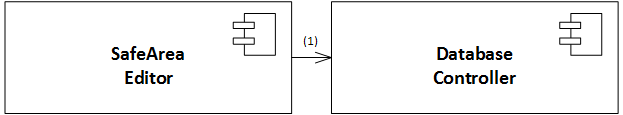
\includegraphics[scale=0.5]{SafeArea/SafeArea1}
\centering
\end{figure}
Then we integrate the SafeArea Manager with both the Database Controller and the SafeArea Editor
\begin{figure}[H]
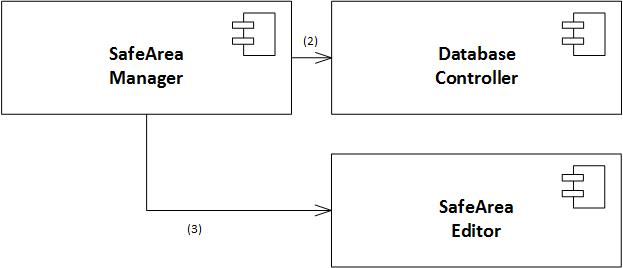
\includegraphics[scale=0.5]{SafeArea/SafeArea2}
\centering
\end{figure}
This is the final integrated subsystem
\begin{figure}[H]
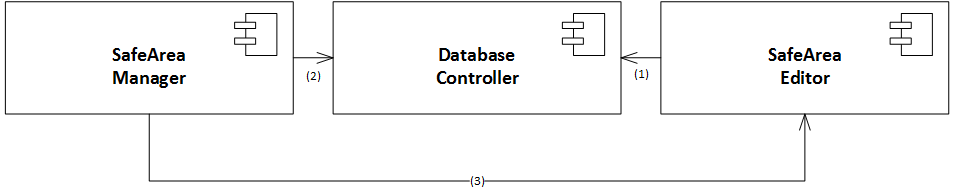
\includegraphics[scale=0.5]{SafeArea/SafeAreaControllerIntegration}
\centering
\end{figure}
\textbf{AssistanceController}
\\
Following a similar procedure as the one used to integrate the SafeArea Controller, we start by testing the interaction between the Assistance List and the Database Controller
\begin{figure}[H]
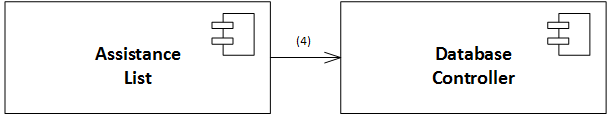
\includegraphics[scale=0.5]{Assistance/Assistance1}
\centering
\end{figure}
We then proceed to integrate the AssistanceList Manager with both the Assistance List and the Notification Forwarder
\begin{figure}[H]
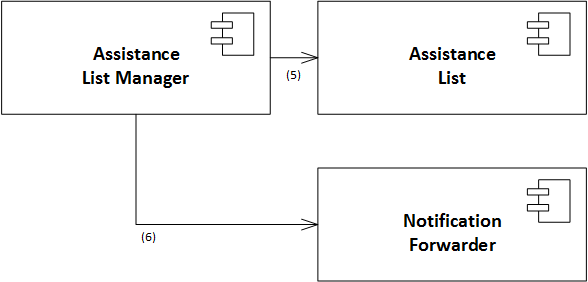
\includegraphics[scale=0.5]{Assistance/Assistance3}
\centering
\end{figure}
This is the final integrated AssistanceController subsystem
\begin{figure}[H]
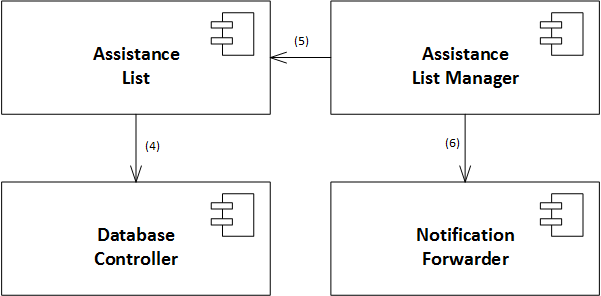
\includegraphics[scale=0.5]{Assistance/AssistanceControllerIntegration}
\centering
\end{figure}
\textbf{EmployeeDispatcher}
\\
Finally, we are able to test all the system together by integrating the EmployeeDispatcher with the two previously tested subsystems
\begin{figure}[H]
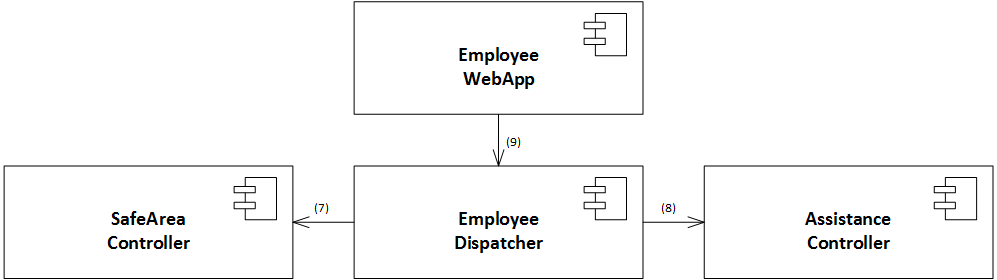
\includegraphics[scale=0.5]{Images/Employee/EmployeeAppIntegration}
\centering
\end{figure}
\newpage

\begin{Large}
\textbf{Car System Strategy}
\end{Large}

In this paragraph we are going to test the System that we will develop for managing the cars. As usual, we are going to follow a bottom-up approach by splitting our system in various subsystem, in order to make testing easier. These are the subsystems we want to test:

\begin{enumerate}
\item CarContoller
\item RideController
\item BillController
\item FaultController
\item FleetController
\item CarApplication
\end{enumerate}

\textbf{CarContoller}
\\
The strategy we will adopt in order to integrate this subsystem is the following: first, we test the Car Data Retriever with the Database Controller and the ECU Data Collector.
\begin{figure}[H]
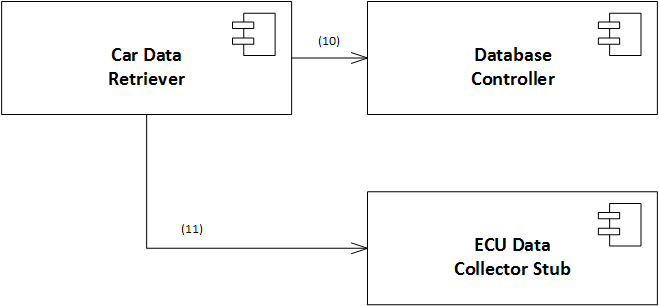
\includegraphics[scale=0.5]{CarController/CarController1}
\centering
\end{figure}
Then we will integrate the Car Actuator Manager with the Car Actuator.
\begin{figure}[H]
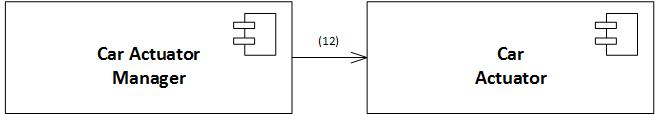
\includegraphics[scale=0.5]{CarController/CarController2}
\centering
\end{figure}
\textbf{RideController}
\\
For the RideController, we first start integrating the Ride Ender with the Bill Manager and the Infraction Manager.
\begin{figure}[H]
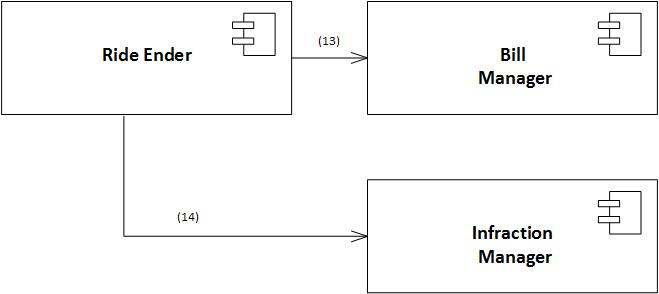
\includegraphics[scale=0.5]{RideController/RideController1}
\centering
\end{figure}
Subsequently, we integrate the Ride Manager with the Car Data Retriever  and, finally, with the Ride Ender that we previously tested
\begin{figure}[H]
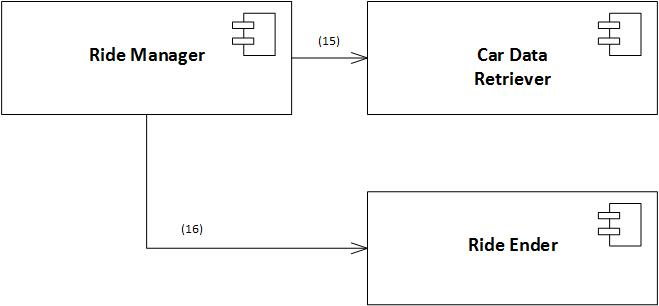
\includegraphics[scale=0.5]{RideController/RideController2}
\centering
\end{figure}
This is the final integrated RideController module
\begin{figure}[H]
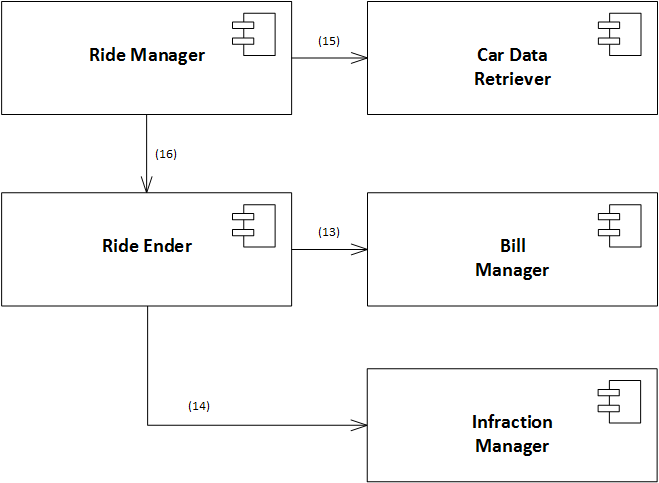
\includegraphics[scale=0.5]{RideController/RideControllerIntegration}
\centering
\end{figure}
\textbf{BillController}
\\
In testing the BillController, we must integrate the Bill Manager with the Balance Manager
\begin{figure}[H]
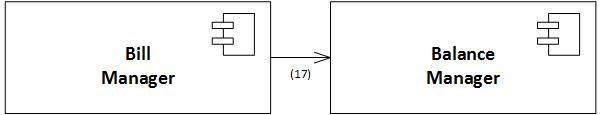
\includegraphics[scale=0.5]{BillController/BillController2}
\centering
\end{figure}
\textbf{FaultController}
\\
The integration sequence of the FaultController is straightforward, since we just need to test the interaction between the Fault Manager and the Assistance List Manager 
\begin{figure}[H]
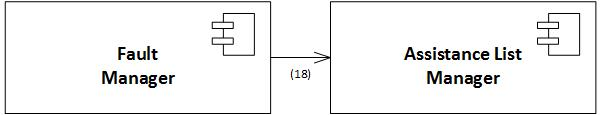
\includegraphics[scale=0.5]{FaultController/FaultController}
\centering
\end{figure}
\textbf{FleetController}
\\
The FleetController simply needs to integrate its own components with the Database Controller. We will first integrate the Registration Manager and then the Dismission Manager
\begin{figure}[H]
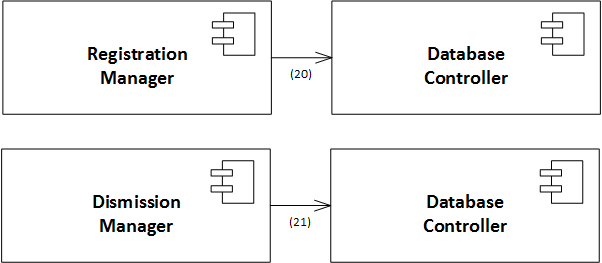
\includegraphics[scale=0.5]{FleetController/FleetController}
\centering
\end{figure}
\textbf{CarApplication}
\\
The CarApplication will be the last module we will test. To do this, we first integrate the Data Analyzer with the ECU Data Collector and the Communication Manager
\begin{figure}[H]
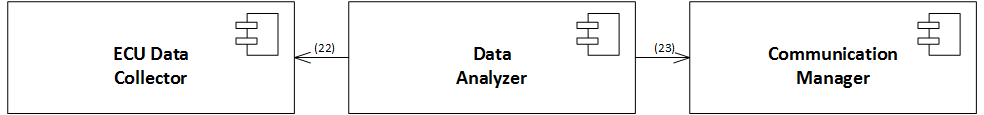
\includegraphics[scale=0.5]{CarApplication/CarApplication1}
\centering
\end{figure}
In the second step, we test the Communication Manager integration with the Car App Dispatcher
\begin{figure}[H]
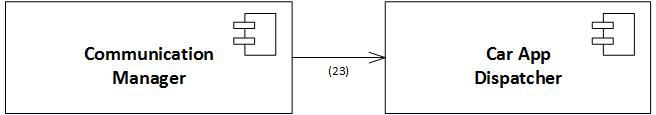
\includegraphics[scale=0.5]{CarApplication/CarApplication2}
\centering
\end{figure}
Finally, we test the interaction between the Fleet Registrator and the Communication Manager
\begin{figure}[H]
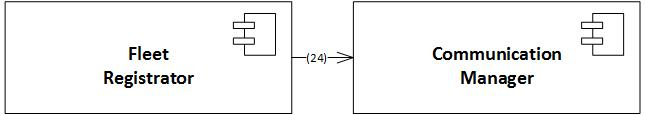
\includegraphics[scale=0.5]{CarApplication/CarApplication3}
\centering
\end{figure}
This is the whole integrated Car Application subsystem
\begin{figure}[H]
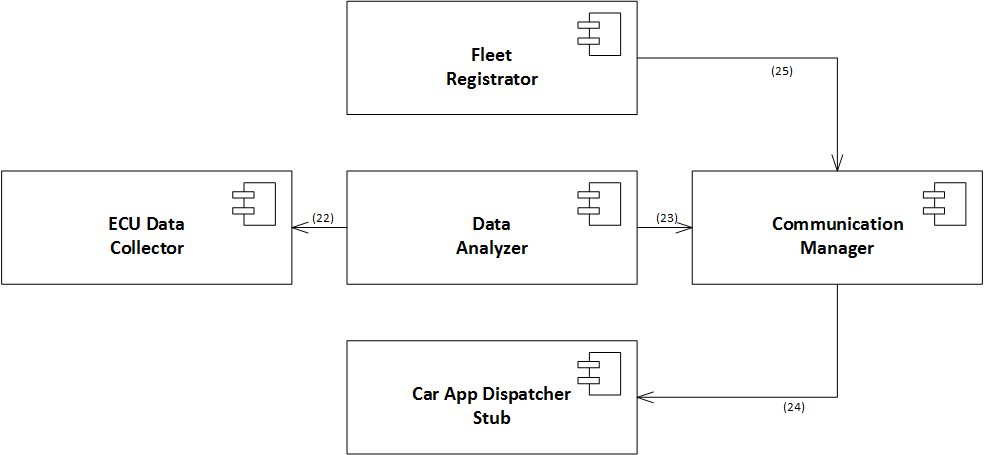
\includegraphics[scale=0.5]{CarApplication/CarApplicationIntegration}
\centering
\end{figure}
\textbf{Modules Integration}
\\
The final step of the Car System integration is to integrate all the modules in the following way
\begin{figure}[H]
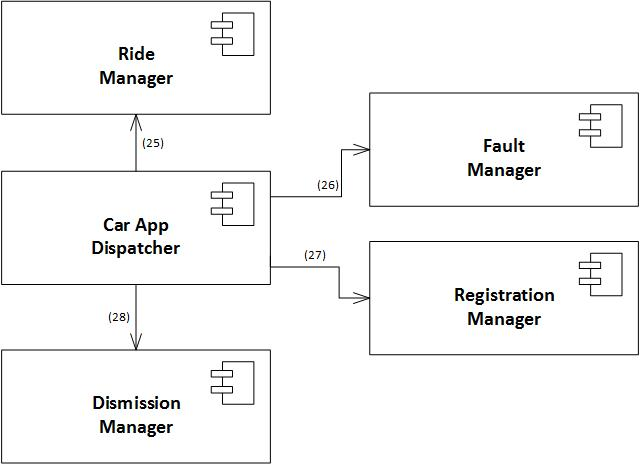
\includegraphics[scale=0.5]{Dispatcher/Dispatcher} 
\centering
\end{figure}

\begin{large}
\textbf{Customer Subsystem}
\end{large}

As aforementioned, we will keep using a bottom-up approach in integating functional groups of the Customer subsystem. We will order them from the most critical module to the least critical. This is the ordering we are going to follow:
\begin{itemize}
\item ReservationController
\item BalanceController
\item AccountController
\item RegistrationController
\item ReportController
\end{itemize}
\begin{Large}
\textbf{ClientDispatcher}
\end{Large}

We will integrate the ClientDispatcher with each one of the previously integrated modules
\begin{figure}[H]
\centering
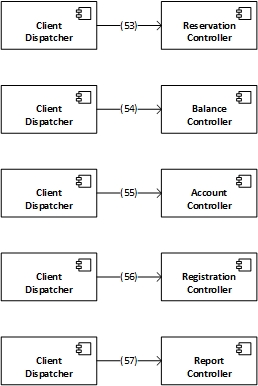
\includegraphics[scale=1]{CustomerDispatcher/Dispatcher_Integration}
\end{figure}

This is the final integrated module
\begin{figure}[H]
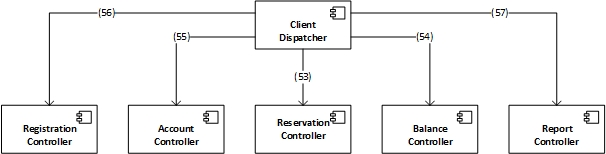
\includegraphics[scale=1]{CustomerDispatcher/Complete_Integration}
\end{figure}

\begin{Large}
\textbf{ClientDispatcher}
\end{Large}

We will integrate the ClientDispatcher with each one of the previously integrated modules
\begin{figure}[H]
\centering
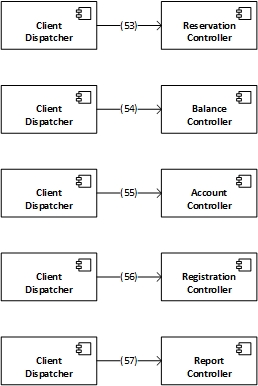
\includegraphics[scale=1]{CustomerDispatcher/Dispatcher_Integration}
\end{figure}

This is the final integrated module
\begin{figure}[H]
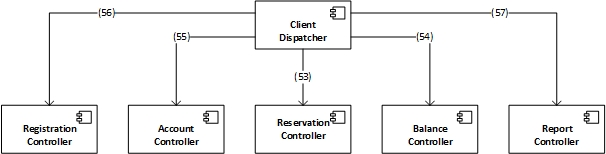
\includegraphics[scale=1]{CustomerDispatcher/Complete_Integration}
\end{figure}

\begin{Large}
\textbf{ClientDispatcher}
\end{Large}

We will integrate the ClientDispatcher with each one of the previously integrated modules
\begin{figure}[H]
\centering
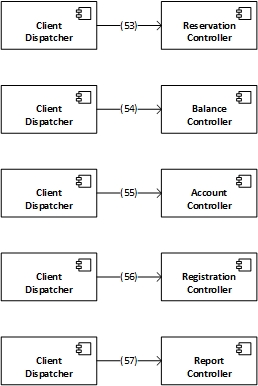
\includegraphics[scale=1]{CustomerDispatcher/Dispatcher_Integration}
\end{figure}

This is the final integrated module
\begin{figure}[H]
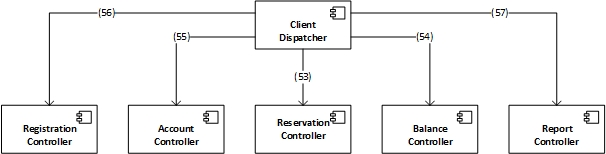
\includegraphics[scale=1]{CustomerDispatcher/Complete_Integration}
\end{figure}

\begin{Large}
\textbf{ClientDispatcher}
\end{Large}

We will integrate the ClientDispatcher with each one of the previously integrated modules
\begin{figure}[H]
\centering
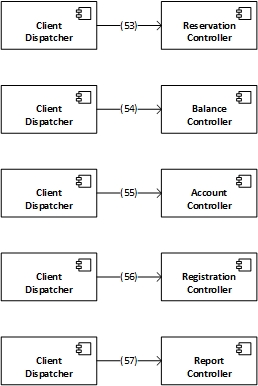
\includegraphics[scale=1]{CustomerDispatcher/Dispatcher_Integration}
\end{figure}

This is the final integrated module
\begin{figure}[H]
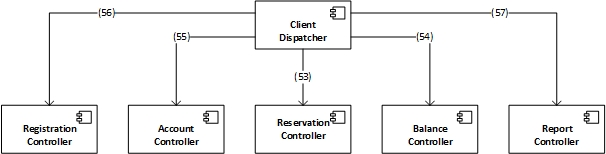
\includegraphics[scale=1]{CustomerDispatcher/Complete_Integration}
\end{figure}

\begin{Large}
\textbf{ClientDispatcher}
\end{Large}

We will integrate the ClientDispatcher with each one of the previously integrated modules
\begin{figure}[H]
\centering
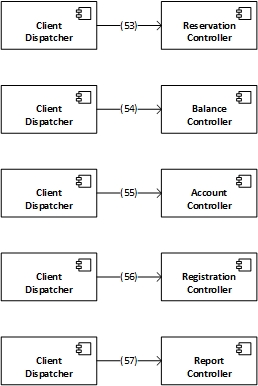
\includegraphics[scale=1]{CustomerDispatcher/Dispatcher_Integration}
\end{figure}

This is the final integrated module
\begin{figure}[H]
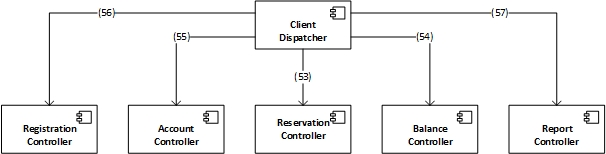
\includegraphics[scale=1]{CustomerDispatcher/Complete_Integration}
\end{figure}

\begin{Large}
\textbf{ClientDispatcher}
\end{Large}

We will integrate the ClientDispatcher with each one of the previously integrated modules
\begin{figure}[H]
\centering
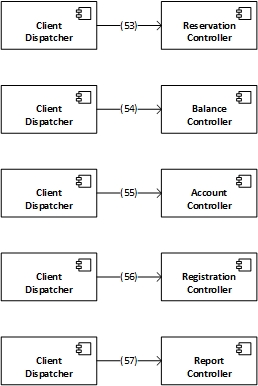
\includegraphics[scale=1]{CustomerDispatcher/Dispatcher_Integration}
\end{figure}

This is the final integrated module
\begin{figure}[H]
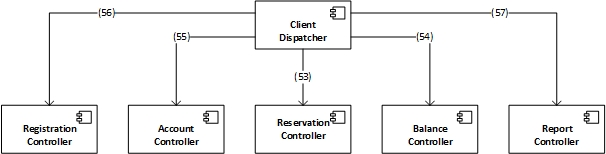
\includegraphics[scale=1]{CustomerDispatcher/Complete_Integration}
\end{figure}

\subsubsection{Subsystem Integration Sequence}
To integrate the tested subsystem, we start from integrating the Customer subsystem with the Employee Subsystem

\begin{figure}[H]
\centering
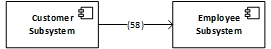
\includegraphics[scale=1]{Subsystems/Customer_employee}
\end{figure}

Then we proceed integrating the Customer subsystem with the car subsystem
\begin{figure}[H]
\centering
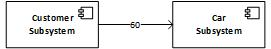
\includegraphics[scale=1]{Subsystems/Customer_car}
\end{figure}

And the other way around
\begin{figure}[H]
\centering
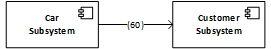
\includegraphics[scale=1]{Subsystems/Car_customer}
\end{figure}

To end the process, we integrate the Car subsystem with the employee subsystem
\begin{figure}[H]
\centering
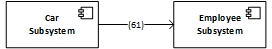
\includegraphics[scale=1]{Subsystems/Car_employee}
\end{figure}

This is the final integrated system
\begin{figure}[H]
\centering
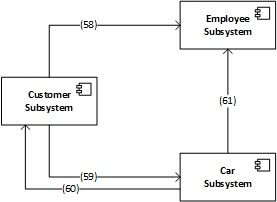
\includegraphics[scale=1]{Subsystems/Integration}
\end{figure}

\newpage
\section{Individual Steps and Test Description}
\subsection{Employee Subsystem}
\subsubsection{I1 Safe Area Editor - Database Controller}
\begin{tabular}{ |p{5cm}|p{7cm}| }
  \hline
  \multicolumn{2}{|c|}{create-safe-area(boundaries)} \\
  \hline
  \textbf{Input} & \textbf{Effect} \\
  \hline
  Null parameter & NullArgumentException is raised\\
  \hline
  Empty list & InvalidArgumentValueException is raised\\
  \hline
  List containing some Null values & NullArgumentException is raised\\
  \hline
  List containing some out-of-bound boundaries (i.e. inexistent coordinates) & OutOfBoundException is raised\\
  \hline
  List containing some coordinates which are already in an existing safe area & Overlap Exception is raised\\
  \hline
  List containing all valid boundaries & The database is updated to include the new safe area\\
  \hline
\end{tabular}
\subsubsection{I2 Safe Area Manager - Database Controller}
\begin{tabular}{ |p{5cm}|p{7cm}| }
  \hline
  \multicolumn{2}{|c|}{get-safe-areas()} \\
  \hline
  \textbf{Input} & \textbf{Effect} \\
  \hline
  Nothing & Return a list of all the safe areas\\
  \hline
\end{tabular}
\subsubsection{I4 Assitance List - Database Controller}
\begin{tabular}{ |p{5cm}|p{7cm}| }
  \hline
  \multicolumn{2}{|c|}{add(vehicle-id)} \\
  \hline
  \textbf{Input} & \textbf{Effect} \\
  \hline
  Null parameter & NullArgumentException is raised\\
  \hline
  Vehicle already present in the assistance list & AlreadyNeedyException is raised\\
  \hline
  Vehicle that is not in the database (i.e. it has not been registered in the fleet) & InvalidVehicleException is raised\\
  \hline
  Valid vehicle & Add the vehicle to the assistance list and sets it as unavailable\\
  \hline
\end{tabular}
\newline
\begin{tabular}{ |p{5cm}|p{7cm}| }
  \hline
  \multicolumn{2}{|c|}{solved(vehicle-id)} \\
  \hline
  \textbf{Input} & \textbf{Effect} \\
  \hline
  Null parameter & NullArgumentException is raised\\
  \hline
  Vehicle that is not in the assistance list & NotNeedyVehicleException is raised\\
  \hline
  Vehicle that is not in the database (i.e. it has not been registered in the fleet) & InvalidVehicleException is raised\\
  \hline
  Valid vehicle & Delete the vehicle from the assistance list and sets it as available\\
  \hline
\end{tabular}
\newline
\begin{tabular}{ |p{5cm}|p{7cm}| }
  \hline
  \multicolumn{2}{|c|}{get-needy-vehicles()} \\
  \hline
  \textbf{Input} & \textbf{Effect} \\
  \hline
  Nothing & Return a list of all the vehicles that need assistance\\
  \hline
\end{tabular}
\begin{tabular}{ |p{5cm}|p{7cm}| }
  \hline
  \multicolumn{2}{|c|}{take-in-charge(vehicle-id,employee-id)} \\
  \hline
  \textbf{Input} & \textbf{Effect} \\
  \hline
  Any of the two is a Null parameter & NullArgumentException is raised\\
  \hline
 Vehicle that is not in the database (i.e. it has not been registered in the fleet), Any & InvalidVehicleException is raised\\
  \hline
  Any, Invalid employee-id & InvalidEmployeeException is raised\\
  \hline
  Vehicle that is not in the assistance list (e.g. it has already been taken in charge by another employee), Any & NotNeedyVehicleException is raised\\
  \hline
  Valid vehicle, valid employee-id & Remove the vehicle from the assistance list and assigns it to that employee\\
  \hline
\end{tabular}
\subsubsection{I5 Assistance List Manager - Assistance List}
\begin{tabular}{ |p{5cm}|p{7cm}| }
  \hline
  \multicolumn{2}{|c|}{addVehicle(vehicle-id)} \\
  \hline
  \textbf{Input} & \textbf{Effect} \\
  \hline
  Null parameter & NullArgumentException is raised\\
  \hline
  Vehicle already present in the assistance list & AlreadyNeedyException is raised\\
  \hline
  Vehicle that is not in the database (i.e. it has not been registered in the fleet) & InvalidArgumentException is raised\\
  \hline
  Valid vehicle & Add the vehicle to the assistance list and sets it as unavailable\\
  \hline
\end{tabular}
\subsubsection{I6 Assitance List Manager - Notification Forwarder}
\begin{tabular}{ |p{5cm}|p{7cm}| }
  \hline
  \multicolumn{2}{|c|}{notify(user,info)} \\
  \hline
  \textbf{Input} & \textbf{Effect} \\
  \hline
   Any of the two is a Null parameter & NullArgumentException is raised\\
  \hline
 User cannot be reached, Any & FailedCommunicationException is raised\\
  \hline
  Valid user, Valid info & A notification containing the specified info is sent to the specified user\\
  \hline
\end{tabular}
\subsubsection{I7 Employee Dispatcher - Safe Area Controller}
\begin{tabular}{ |p{5cm}|p{7cm}| }
  \hline
  \multicolumn{2}{|c|}{create-safe-area(boundaries)} \\
  \hline
  \textbf{Input} & \textbf{Effect} \\
  \hline
  Null parameter & NullArgumentException is raised\\
  \hline
  Empty list & InvalidArgumentValueException is raised\\
  \hline
  List containing some Null values & NullArgumentException is raised\\
  \hline
  List containing some out-of-bound boundaries (i.e. inexistent coordinates) & OutOfBoundException is raised\\
  \hline
  List containing some coordinates which are already in an existing safe area & Overlap Exception is raised\\
  \hline
  List containing all valid boundaries & The database is updated to include the new safe area\\
  \hline
\end{tabular}
\newline
\begin{tabular}{ |p{5cm}|p{7cm}| }
  \hline
  \multicolumn{2}{|c|}{get-safe-areas()} \\
  \hline
  \textbf{Input} & \textbf{Effect} \\
  \hline
  Nothing & Return a list of all the safe areas\\
  \hline
\end{tabular}
\subsubsection{I8 Employee Dispatcher - Assistance Controller}
\begin{tabular}{ |p{5cm}|p{7cm}| }
  \hline
  \multicolumn{2}{|c|}{solved(vehicle-id)} \\
  \hline
  \textbf{Input} & \textbf{Effect} \\
  \hline
  Null parameter & NullArgumentException is raised\\
  \hline
  Vehicle that is not in the assistance list & NotNeedyVehicleException is raised\\
  \hline
  Vehicle that is not in the database (i.e. it has not been registered in the fleet) & InvalidVehicleException is raised\\
  \hline
  Valid vehicle & Delete the vehicle from the assistance list and sets it as available\\
  \hline
\end{tabular}
\newline
\begin{tabular}{ |p{5cm}|p{7cm}| }
  \hline
  \multicolumn{2}{|c|}{get-needy-vehicles()} \\
  \hline
  \textbf{Input} & \textbf{Effect} \\
  \hline
  Nothing & Return a list of all the vehicles that need assistance\\
  \hline
\end{tabular}
\newline
\begin{tabular}{ |p{5cm}|p{7cm}| }
  \hline
  \multicolumn{2}{|c|}{take-in-charge(vehicle-id,employee-id)} \\
  \hline
  \textbf{Input} & \textbf{Effect} \\
  \hline
  Any of the two is a Null parameter & NullArgumentException is raised\\
  \hline
 Vehicle that is not in the database (i.e. it has not been registered in the fleet), Any & InvalidVehicleException is raised\\
  \hline
  Any, Invalid employee-id & InvalidEmployeeException is raised\\
  \hline
  Vehicle that is not in the assistance list (e.g. it has already been taken in charge by another employee), Any & NotNeedyVehicleException is raised\\
  \hline
  Valid vehicle, valid employee-id & Remove the vehicle from the assistance list and assigns it to that employee\\
  \hline
\end{tabular}
\subsubsection{I9 Employee WebApp - Employee Dispatcher}
\begin{tabular}{ |p{5cm}|p{7cm}| }
  \hline
  \multicolumn{2}{|c|}{dispatch-request(request-info)} \\
  \hline
  \textbf{Input} & \textbf{Effect} \\
  \hline
  Null parameter & NullArgumentException is raised\\
  \hline
  Invalid request & InvalidArgumentException is raised \\
  \hline
  Valid request & Forwards employee's request to the dedicated component\\
  \hline
\end{tabular}
\subsection{Car Subsystem}
\subsubsection{I10 Car Data Retriever - Database Controller}
\begin{tabular}{ |p{5cm}|p{7cm}| }
  \hline
  \multicolumn{2}{|c|}{update-car-data(data-type, vehicle-id)} \\
  \hline
  \textbf{Input} & \textbf{Effect} \\
  \hline
  Any of the two is a Null parameter & NullArgumentException is raised\\
  \hline
  Invalid data-type, Any & InvalidArgumentException is raised\\
  \hline
  Any, Vehicle that is not in the database (i.e. it has not been registered in the fleet) & InvalidArgumentException is raised\\
  \hline
   Valid data-type, Valid vehicle-id & Updates car data in the database\\
  \hline
\end{tabular}
\newline
\begin{tabular}{ |p{5cm}|p{7cm}| }
  \hline
  \multicolumn{2}{|c|}{get-car-data(data-type, vehicle-id)} \\
  \hline
  \textbf{Input} & \textbf{Effect} \\
  \hline
  Any of the two is a Null parameter & NullArgumentException is raised\\
  \hline
  Invalid data-type, Any & InvalidArgumentException is raised\\
  \hline
  Any, Vehicle that is not in the database (i.e. it has not been registered in the fleet) & InvalidArgumentException is raised\\
  \hline
   Valid data-type, Valid vehicle-id & Returns the requested data getting it from the database\\
  \hline
\end{tabular}
\subsubsection{I11 Car Data Retriever - ECU Data Collector}
\begin{tabular}{ |p{5cm}|p{7cm}| }
  \hline
  \multicolumn{2}{|c|}{get-data(data-type)} \\
  \hline
  \textbf{Input} & \textbf{Effect} \\
  \hline
  Null parameter & NullArgumentException is raised\\
  \hline
  Invalid data-type & InvalidArgumentException is raised\\
  \hline
  Valid data-type but cannot communicate with the vehicle & FailedComumunicationException is raised\\
  \hline
   Valid data-type & Dialogs with the on-board car application to get the specified data\\
  \hline
\end{tabular}
\subsubsection{I12 Car Actuator Manager - Car Actuator}
\begin{tabular}{ |p{5cm}|p{7cm}| }
  \hline
  \multicolumn{2}{|c|}{unlock()} \\
  \hline
  \textbf{Input} & \textbf{Effect} \\
  \hline
  Nothing but the communication with the car fails & FailedCommunicationException is raised\\
  \hline
  Nothing & The car is unlocked \\
  \hline
\end{tabular}
\subsubsection{I13 Ride Ender - Bill Manager}
\begin{tabular}{ |p{5cm}|p{7cm}| }
  \hline
  \multicolumn{2}{|c|}{calculate-bill(ride-info)} \\
  \hline
  \textbf{Input} & \textbf{Effect} \\
  \hline
  Null parameter & NullArgumentException is raised\\
  \hline
  Invalid ride-info & InvalidArgumentException is raised \\
  \hline
  Vaild ride-info & Calculate the amount of the bill\\
  \hline
\end{tabular}
\subsubsection{I14 Ride Ender - Infraction Manager}
\begin{tabular}{ |p{5cm}|p{7cm}| }
  \hline
  \multicolumn{2}{|c|}{signal-infraction(infraction-info)} \\
  \hline
  \textbf{Input} & \textbf{Effect} \\
  \hline
  Null parameter & NullArgumentException is raised\\
  \hline
  Invalid infraction-info & InvalidArgumentException is raised \\
  \hline
  Vaild infraction-info & Change the user's status as signalled in the database\\
  \hline
\end{tabular}
\subsubsection{I15 Ride Manager - Car Data Retriever }
\begin{tabular}{ |p{5cm}|p{7cm}| }
  \hline
  \multicolumn{2}{|c|}{get-car-data(data-type, vehicle-id)} \\
  \hline
  \textbf{Input} & \textbf{Effect} \\
  \hline
  Any of the two is a Null parameter & NullArgumentException is raised\\
  \hline
  Invalid data-type, Any & InvalidArgumentException is raised\\
  \hline
  Any, Vehicle that is not in the database (i.e. it has not been registered in the fleet) & InvalidArgumentException is raised\\
  \hline
   Valid data-type, Valid vehicle-id & Returns the specified data and updates the database\\
  \hline
\end{tabular}
\subsubsection{I17 Bill Manager - Balance Manager }
\begin{tabular}{ |p{5cm}|p{7cm}| }
  \hline
  \multicolumn{2}{|c|}{pay(amount,user)} \\
  \hline
  \textbf{Input} & \textbf{Effect} \\
  \hline
  Any of the two is a Null parameter & NullArgumentException is raised\\
  \hline
  Invalid amount(e.g. negative value), Any & InvalidArgumentException is raised\\
  \hline
  Any, User that is not in the database & InvalidArgumentException is raised\\
  \hline
   Valid amount, Valid user & The amount is subracted from the user balance\\
  \hline
\end{tabular}
\subsubsection{I18 Fault Manager - Assistant List Manager}
\begin{tabular}{ |p{5cm}|p{7cm}| }
  \hline
  \multicolumn{2}{|c|}{add(vehicle-id)} \\
  \hline
  \textbf{Input} & \textbf{Effect} \\
  \hline
  Null parameter & NullArgumentException is raised\\
  \hline
  Vehicle already present in the assistance list & AlreadyNeedyException is raised\\
  \hline
  Vehicle that is not in the database (i.e. it has not been registered in the fleet) & InvalidArgumentException is raised\\
  \hline
  Valid vehicle & Add the vehicle to the assistance list and sets it as unavailable\\
  \hline
\end{tabular}
\subsubsection{I19 Registration Manager - Database Controller }
\begin{tabular}{ |p{5cm}|p{7cm}| }
  \hline
  \multicolumn{2}{|c|}{register-car(car-info)} \\
  \hline
  \textbf{Input} & \textbf{Effect} \\
  \hline
  Null parameter & NullArgumentException is raised\\
  \hline
  Vehicle already present in the database & AlreadyRegisteredVehicleException is raised\\
  \hline
  Invalid car-info (e.g. vehicle plate too long) & InvalidArgumentException is raised\\
  \hline
  Valid car-info & Add the vehicle to the database and to the fleet\\
  \hline
\end{tabular}
\subsubsection{I20 Dismission Manager - Database Controller }
\begin{tabular}{ |p{5cm}|p{7cm}| }
  \hline
  \multicolumn{2}{|c|}{dismiss-car(car-info)} \\
  \hline
  \textbf{Input} & \textbf{Effect} \\
  \hline
  Null parameter & NullArgumentException is raised\\
  \hline
  Vehicle not present in the database & InexistantCarException is raised\\
  \hline
  Invalid car-info (e.g. vehicle plate too long) & InvalidArgumentException is raised\\
  \hline
  Valid car-info & Dismiss the vehicle from the fleet and delete it from the database\\
  \hline
\end{tabular}
\subsubsection{I21 Data Analyzer - ECU Data Collector}
\begin{tabular}{ |p{5cm}|p{7cm}| }
  \hline
  \multicolumn{2}{|c|}{get-data(data-type)} \\
  \hline
  \textbf{Input} & \textbf{Effect} \\
  \hline
  Null parameter & NullArgumentException is raised\\
  \hline
  Invalid data-type & InvalidArgumentException is raised\\
  \hline
   Valid data-type & Get the specified data from the ECU Data Collector\\
  \hline
\end{tabular}
\subsubsection{I22 Data Analyzer - Communication Manager}
\begin{tabular}{ |p{5cm}|p{7cm}| }
  \hline
  \multicolumn{2}{|c|}{send-fault()} \\
  \hline
  \textbf{Input} & \textbf{Effect} \\
  \hline
  Nothing but the communication fails & FailedCommunicationException is raised\\
  \hline
  Nothing & A fault notification is sent\\
  \hline
\end{tabular}
\subsubsection{I23 Communication Manager - Car App Dispatcher}
\begin{tabular}{ |p{5cm}|p{7cm}| }
  \hline
  \multicolumn{2}{|c|}{dispatch-request(request-info)} \\
  \hline
  \textbf{Input} & \textbf{Effect} \\
  \hline
  Null parameter & NullArgumentException is raised\\
  \hline
  Invalid request & InvalidArgumentException is raised \\
  \hline
  Valid request & Forwards the car application request to the dedicated component\\
  \hline
\end{tabular}
\subsubsection{I24 Fleet Registrator - Communication Manager}
\begin{tabular}{ |p{5cm}|p{7cm}| }
  \hline
  \multicolumn{2}{|c|}{send-registration-request(vehicle-info)} \\
  \hline
  \textbf{Input} & \textbf{Effect} \\
  \hline
  Invalid vehicle-info & InvalidArgumentException is raised\\
  \hline
  Valid vehicle-info but the communication fails & FailedCommunicationException is raised\\
  \hline
  Nothing & A registration request is sent\\
  \hline
\end{tabular}
\subsubsection{I25 Car App Dispatcher - Ride Manager}
\begin{tabular}{ |p{5cm}|p{7cm}| }
  \hline
  \multicolumn{2}{|c|}{start-ride(vehicle-id)} \\
  \hline
  \textbf{Input} & \textbf{Effect} \\
  \hline
   Null parameter & NullArgumentException is raised\\
  \hline
  Valid vehicle-id but communication fails & FailedCommunicationException is raised\\
  \hline
 Valid vehicle-id & The Ride Monitor is aware of the fact that the ride started \\
  \hline
\end{tabular}
\begin{tabular}{ |p{5cm}|p{7cm}| }
  \hline
  \multicolumn{2}{|c|}{end-ride(ride-info)} \\
  \hline
  \textbf{Input} & \textbf{Effect} \\
  \hline
   Null parameter & NullArgumentException is raised\\
  \hline
  invalid ride-info (e.g. negative number of passengers) & InvalidArgumentException is raised\\
  \hline
  Valid ride-info but communication fails & FailedCommunicationException is raised\\
  \hline
 Valid ride-info & The Ride Monitor is aware of the fact that the ride ended, calculate the bill and forward it to the dedicated component \\
  \hline
\end{tabular}
\subsubsection{I26 Car App Dispatcher - Fault Manager}
\begin{tabular}{ |p{5cm}|p{7cm}| }
  \hline
  \multicolumn{2}{|c|}{notify-fault(fault-info)} \\
  \hline
  \textbf{Input} & \textbf{Effect} \\
  \hline
  Null parameter & NullArgumentException is raised\\
  \hline
  Valid fault-info but failed communication & FailedCommunicationException is raised\\
  \hline
  Valid fault-info & Forwards the fault-info to the employee system by means of a notification\\
  \hline
\end{tabular}
\subsubsection{I27 Car App Dispatcher - Registration Manager}
\begin{tabular}{ |p{5cm}|p{7cm}| }
  \hline
  \multicolumn{2}{|c|}{register-car(car-info)} \\
  \hline
  \textbf{Input} & \textbf{Effect} \\
  \hline
  Null parameter & NullArgumentException is raised\\
  \hline
  Vehicle already present in the database & AlreadyRegisteredVehicleException is raised\\
  \hline
  Invalid car-info (e.g. vehicle plate too long) & InvalidArgumentException is raised\\
  \hline
  Valid car-info & Add the vehicle to the database and to the fleet\\
  \hline
\end{tabular}
\subsubsection{I28 Car App Dispatcher - Dismission Manager}
\begin{tabular}{ |p{5cm}|p{7cm}| }
  \hline
  \multicolumn{2}{|c|}{dismiss-car(car-info)} \\
  \hline
  \textbf{Input} & \textbf{Effect} \\
  \hline
  Null parameter & NullArgumentException is raised\\
  \hline
  Vehicle not present in the database & InexistantCarException is raised\\
  \hline
  Invalid car-info (e.g. vehicle plate too long) & InvalidArgumentException is raised\\
  \hline
  Valid car-info & Dismiss the vehicle from the fleet and delete it from the database\\
  \hline
\end{tabular}

\subsection{Customer Subsystem}
\subsubsection{ClientDispatcher, ReservationController}

\begin{tabular}{|p{5cm}|p{7cm}|}
\hline
\multicolumn{2}{|c|}{reserve(vehicle-id, user)} \\
\hline
\textbf{Input} & \textbf{Effect} \\

\hline
A Null parameter & NullParameterException is raised \\

\hline
Any, Non existing user & InvalidArgumentException is raised \\
\hline
Non existing vehicle, Existing user & InvalidArgumentException is raised \\

\hline
Debtor user, Any & InvalidUserException is raised \\

\hline
Banned user, Any & InvalidUserException is raised \\

\hline
Regular user, Reserved vehicle  & UnavailableCarException is raised \\

\hline
Regular user, Needy vehicle & UnavailableCarException is raised \\

\hline
Regular user, Available vehicle & Database entry is created \\
\hline
\end{tabular}
\\
\begin{tabular}{|p{5cm}|p{7cm}|}
\hline
\multicolumn{2}{|c|}{unlock(veicle-id, user)} \\
\hline
\textbf{Input} & \textbf{Effect} \\

\hline
A Null parameter & NullParameterException is raised \\

\hline
Non existing vehicle, Any & InvalidVehicleException is raised \\

\hline
Existing vehicle, user too far from the car & TooFarException is raised \\

\hline
Existing but unlocked vehicle, valid user-info & AlreadyUnlockedException is raised \\

\hline
Existing and locked vehicle, valid user-info & Database entry is updated, reservation timer is stopped and car is unlocked \\
\hline
\end{tabular}
\\
\begin{tabular}{|p{5cm}|p{7cm}|}
\hline
\multicolumn{2}{|c|}{get-near-vehicles(position)} \\
\hline
\textbf{Input} & \textbf{Effect} \\

\hline
A Null parameter & NullParameterException is raised \\

\hline
Invalid position, Any & InvalidPositionException is raised \\

\hline
Valid position, Non-positive integer & InvalidArgmuentException is raised \\

\hline
Valid position, Positive integer & Returns the list of available cars in the input range from the input poition \\
\hline
\end{tabular}
\subsubsection{ClientDispatcher, BalanceController}
\begin{tabular}{|p{5cm}|p{7cm}|}
\hline
\multicolumn{2}{|c|}{deposit(payment-method, amount, user-id} \\
\hline
\textbf{Input} & \textbf{Effect} \\

\hline
A Null parameter & NullParameterException is raised \\

\hline
Any, Any, Non existing user & InvalidUserException is raised \\

\hline
Invalid info, Any, Existing user & TransactionExeption is raised \\

\hline
Valid info, Non-positive value, Existing user & InvalidArgumentException is raised \\

\hline
Valid info, Positive value more than affordable, Existing user & TransactionException is raised \\

\hline
Valid info, Positive value less than affordable, Existing user & Money is transfered from user payment provider to the company \\
\hline
\end{tabular}
\subsubsection{ClientDispatcher, AccountController}
\begin{tabular}{|p{5cm}|p{7cm}|}
\hline
\multicolumn{2}{|c|}{login(username, password)} \\
\hline
\textbf{Input} & \textbf{Effect} \\

\hline
A Null parameter & NullParameterException is raised \\

\hline
Non existing user, Any & InvalidCredentialException is raised \\

\hline
Existing user, Wrong password & InvalidCredentialException is raised \\

\hline
Existing user, Correct password & Login is granted \\
\hline
\end{tabular}
\\
\begin{tabular}{|p{5cm}|p{7cm}|}
\hline
\multicolumn{2}{|c|}{get-personal-info(user-id)} \\
\hline
\textbf{Input} & \textbf{Effect} \\

\hline
A Null parameter & NullParameterException is raised \\

\hline
Non existing user & InvalidUserException is raised \\

\hline
Existing user & Returns user’s information from the database \\
\hline
\end{tabular}
\\
\begin{tabular}{|p{5cm}|p{7cm}|}
\hline
\multicolumn{2}{|c|}{edit-personal-info(user-info, user-id)} \\
\hline
\textbf{Input} & \textbf{Effect} \\

\hline
A Null parameter & NullParameterException is raised \\

\hline
Any, Non existing user & InvalidArgumentException is raised \\

\hline
Invalid payment info, Existing user & InvalidPaymentInfoException is raised \\

\hline
Invalid driving license, Existing user & InvalidLicenseException is raised \\

\hline
Valid info, Existing user & Database entries are updated \\
\hline
\end{tabular}

\subsubsection{ClientDispatcher, RegistrationController}
\begin{tabular}{|p{5cm}|p{7cm}|}
\hline
\multicolumn{2}{|c|}{register(user-info)} \\
\hline
\textbf{Input} & \textbf{Effect} \\

\hline
A Null parameter & NullParameterException is raised \\

\hline
Invalid payment info & InvalidPaymentInfoException is raised \\

\hline
Invalid driving license & InvalidLicenseException is raised \\

\hline
Existing username & AlreadyExistingUsernameException is raised \\

\hline
New username, Valid info & Database entry is created \\
\hline
\end{tabular}
\subsubsection{ClientDispatcher, ReportController}

\begin{tabular}{|p{5cm}|p{7cm}|}
\hline
\multicolumn{2}{|c|}{report(vehicle-plate, report)} \\
\hline
\textbf{Input} & \textbf{Effect} \\

\hline
A Null parameter & NullParameterException is raised \\

\hline
Non existing plate, Any & InvalidArgumentException is raised \\

\hline
Valid plate, Empty report & InvalidArgumentException is raised \\

\hline
Valid plate, Non-empty report & Database entry is created and vehicle is added to AssistanceList\\
\hline
\end{tabular}
\subsubsection{ClientDispatcher, ReservationController}

\begin{tabular}{|p{5cm}|p{7cm}|}
\hline
\multicolumn{2}{|c|}{reserve(vehicle-id, user)} \\
\hline
\textbf{Input} & \textbf{Effect} \\

\hline
A Null parameter & NullParameterException is raised \\

\hline
Any, Non existing user & InvalidArgumentException is raised \\
\hline
Non existing vehicle, Existing user & InvalidArgumentException is raised \\

\hline
Debtor user, Any & InvalidUserException is raised \\

\hline
Banned user, Any & InvalidUserException is raised \\

\hline
Regular user, Reserved vehicle  & UnavailableCarException is raised \\

\hline
Regular user, Needy vehicle & UnavailableCarException is raised \\

\hline
Regular user, Available vehicle & Database entry is created \\
\hline
\end{tabular}
\\
\begin{tabular}{|p{5cm}|p{7cm}|}
\hline
\multicolumn{2}{|c|}{unlock(veicle-id, user)} \\
\hline
\textbf{Input} & \textbf{Effect} \\

\hline
A Null parameter & NullParameterException is raised \\

\hline
Non existing vehicle, Any & InvalidVehicleException is raised \\

\hline
Existing vehicle, user too far from the car & TooFarException is raised \\

\hline
Existing but unlocked vehicle, valid user-info & AlreadyUnlockedException is raised \\

\hline
Existing and locked vehicle, valid user-info & Database entry is updated, reservation timer is stopped and car is unlocked \\
\hline
\end{tabular}
\\
\begin{tabular}{|p{5cm}|p{7cm}|}
\hline
\multicolumn{2}{|c|}{get-near-vehicles(position)} \\
\hline
\textbf{Input} & \textbf{Effect} \\

\hline
A Null parameter & NullParameterException is raised \\

\hline
Invalid position, Any & InvalidPositionException is raised \\

\hline
Valid position, Non-positive integer & InvalidArgmuentException is raised \\

\hline
Valid position, Positive integer & Returns the list of available cars in the input range from the input poition \\
\hline
\end{tabular}
\subsubsection{ClientDispatcher, BalanceController}
\begin{tabular}{|p{5cm}|p{7cm}|}
\hline
\multicolumn{2}{|c|}{deposit(payment-method, amount, user-id} \\
\hline
\textbf{Input} & \textbf{Effect} \\

\hline
A Null parameter & NullParameterException is raised \\

\hline
Any, Any, Non existing user & InvalidUserException is raised \\

\hline
Invalid info, Any, Existing user & TransactionExeption is raised \\

\hline
Valid info, Non-positive value, Existing user & InvalidArgumentException is raised \\

\hline
Valid info, Positive value more than affordable, Existing user & TransactionException is raised \\

\hline
Valid info, Positive value less than affordable, Existing user & Money is transfered from user payment provider to the company \\
\hline
\end{tabular}
\subsubsection{ClientDispatcher, AccountController}
\begin{tabular}{|p{5cm}|p{7cm}|}
\hline
\multicolumn{2}{|c|}{login(username, password)} \\
\hline
\textbf{Input} & \textbf{Effect} \\

\hline
A Null parameter & NullParameterException is raised \\

\hline
Non existing user, Any & InvalidCredentialException is raised \\

\hline
Existing user, Wrong password & InvalidCredentialException is raised \\

\hline
Existing user, Correct password & Login is granted \\
\hline
\end{tabular}
\\
\begin{tabular}{|p{5cm}|p{7cm}|}
\hline
\multicolumn{2}{|c|}{get-personal-info(user-id)} \\
\hline
\textbf{Input} & \textbf{Effect} \\

\hline
A Null parameter & NullParameterException is raised \\

\hline
Non existing user & InvalidUserException is raised \\

\hline
Existing user & Returns user’s information from the database \\
\hline
\end{tabular}
\\
\begin{tabular}{|p{5cm}|p{7cm}|}
\hline
\multicolumn{2}{|c|}{edit-personal-info(user-info, user-id)} \\
\hline
\textbf{Input} & \textbf{Effect} \\

\hline
A Null parameter & NullParameterException is raised \\

\hline
Any, Non existing user & InvalidArgumentException is raised \\

\hline
Invalid payment info, Existing user & InvalidPaymentInfoException is raised \\

\hline
Invalid driving license, Existing user & InvalidLicenseException is raised \\

\hline
Valid info, Existing user & Database entries are updated \\
\hline
\end{tabular}

\subsubsection{ClientDispatcher, RegistrationController}
\begin{tabular}{|p{5cm}|p{7cm}|}
\hline
\multicolumn{2}{|c|}{register(user-info)} \\
\hline
\textbf{Input} & \textbf{Effect} \\

\hline
A Null parameter & NullParameterException is raised \\

\hline
Invalid payment info & InvalidPaymentInfoException is raised \\

\hline
Invalid driving license & InvalidLicenseException is raised \\

\hline
Existing username & AlreadyExistingUsernameException is raised \\

\hline
New username, Valid info & Database entry is created \\
\hline
\end{tabular}
\subsubsection{ClientDispatcher, ReportController}

\begin{tabular}{|p{5cm}|p{7cm}|}
\hline
\multicolumn{2}{|c|}{report(vehicle-plate, report)} \\
\hline
\textbf{Input} & \textbf{Effect} \\

\hline
A Null parameter & NullParameterException is raised \\

\hline
Non existing plate, Any & InvalidArgumentException is raised \\

\hline
Valid plate, Empty report & InvalidArgumentException is raised \\

\hline
Valid plate, Non-empty report & Database entry is created and vehicle is added to AssistanceList\\
\hline
\end{tabular}
\subsubsection{ClientDispatcher, ReservationController}

\begin{tabular}{|p{5cm}|p{7cm}|}
\hline
\multicolumn{2}{|c|}{reserve(vehicle-id, user)} \\
\hline
\textbf{Input} & \textbf{Effect} \\

\hline
A Null parameter & NullParameterException is raised \\

\hline
Any, Non existing user & InvalidArgumentException is raised \\
\hline
Non existing vehicle, Existing user & InvalidArgumentException is raised \\

\hline
Debtor user, Any & InvalidUserException is raised \\

\hline
Banned user, Any & InvalidUserException is raised \\

\hline
Regular user, Reserved vehicle  & UnavailableCarException is raised \\

\hline
Regular user, Needy vehicle & UnavailableCarException is raised \\

\hline
Regular user, Available vehicle & Database entry is created \\
\hline
\end{tabular}
\\
\begin{tabular}{|p{5cm}|p{7cm}|}
\hline
\multicolumn{2}{|c|}{unlock(veicle-id, user)} \\
\hline
\textbf{Input} & \textbf{Effect} \\

\hline
A Null parameter & NullParameterException is raised \\

\hline
Non existing vehicle, Any & InvalidVehicleException is raised \\

\hline
Existing vehicle, user too far from the car & TooFarException is raised \\

\hline
Existing but unlocked vehicle, valid user-info & AlreadyUnlockedException is raised \\

\hline
Existing and locked vehicle, valid user-info & Database entry is updated, reservation timer is stopped and car is unlocked \\
\hline
\end{tabular}
\\
\begin{tabular}{|p{5cm}|p{7cm}|}
\hline
\multicolumn{2}{|c|}{get-near-vehicles(position)} \\
\hline
\textbf{Input} & \textbf{Effect} \\

\hline
A Null parameter & NullParameterException is raised \\

\hline
Invalid position, Any & InvalidPositionException is raised \\

\hline
Valid position, Non-positive integer & InvalidArgmuentException is raised \\

\hline
Valid position, Positive integer & Returns the list of available cars in the input range from the input poition \\
\hline
\end{tabular}
\subsubsection{ClientDispatcher, BalanceController}
\begin{tabular}{|p{5cm}|p{7cm}|}
\hline
\multicolumn{2}{|c|}{deposit(payment-method, amount, user-id} \\
\hline
\textbf{Input} & \textbf{Effect} \\

\hline
A Null parameter & NullParameterException is raised \\

\hline
Any, Any, Non existing user & InvalidUserException is raised \\

\hline
Invalid info, Any, Existing user & TransactionExeption is raised \\

\hline
Valid info, Non-positive value, Existing user & InvalidArgumentException is raised \\

\hline
Valid info, Positive value more than affordable, Existing user & TransactionException is raised \\

\hline
Valid info, Positive value less than affordable, Existing user & Money is transfered from user payment provider to the company \\
\hline
\end{tabular}
\subsubsection{ClientDispatcher, AccountController}
\begin{tabular}{|p{5cm}|p{7cm}|}
\hline
\multicolumn{2}{|c|}{login(username, password)} \\
\hline
\textbf{Input} & \textbf{Effect} \\

\hline
A Null parameter & NullParameterException is raised \\

\hline
Non existing user, Any & InvalidCredentialException is raised \\

\hline
Existing user, Wrong password & InvalidCredentialException is raised \\

\hline
Existing user, Correct password & Login is granted \\
\hline
\end{tabular}
\\
\begin{tabular}{|p{5cm}|p{7cm}|}
\hline
\multicolumn{2}{|c|}{get-personal-info(user-id)} \\
\hline
\textbf{Input} & \textbf{Effect} \\

\hline
A Null parameter & NullParameterException is raised \\

\hline
Non existing user & InvalidUserException is raised \\

\hline
Existing user & Returns user’s information from the database \\
\hline
\end{tabular}
\\
\begin{tabular}{|p{5cm}|p{7cm}|}
\hline
\multicolumn{2}{|c|}{edit-personal-info(user-info, user-id)} \\
\hline
\textbf{Input} & \textbf{Effect} \\

\hline
A Null parameter & NullParameterException is raised \\

\hline
Any, Non existing user & InvalidArgumentException is raised \\

\hline
Invalid payment info, Existing user & InvalidPaymentInfoException is raised \\

\hline
Invalid driving license, Existing user & InvalidLicenseException is raised \\

\hline
Valid info, Existing user & Database entries are updated \\
\hline
\end{tabular}

\subsubsection{ClientDispatcher, RegistrationController}
\begin{tabular}{|p{5cm}|p{7cm}|}
\hline
\multicolumn{2}{|c|}{register(user-info)} \\
\hline
\textbf{Input} & \textbf{Effect} \\

\hline
A Null parameter & NullParameterException is raised \\

\hline
Invalid payment info & InvalidPaymentInfoException is raised \\

\hline
Invalid driving license & InvalidLicenseException is raised \\

\hline
Existing username & AlreadyExistingUsernameException is raised \\

\hline
New username, Valid info & Database entry is created \\
\hline
\end{tabular}
\subsubsection{ClientDispatcher, ReportController}

\begin{tabular}{|p{5cm}|p{7cm}|}
\hline
\multicolumn{2}{|c|}{report(vehicle-plate, report)} \\
\hline
\textbf{Input} & \textbf{Effect} \\

\hline
A Null parameter & NullParameterException is raised \\

\hline
Non existing plate, Any & InvalidArgumentException is raised \\

\hline
Valid plate, Empty report & InvalidArgumentException is raised \\

\hline
Valid plate, Non-empty report & Database entry is created and vehicle is added to AssistanceList\\
\hline
\end{tabular}
\subsubsection{ClientDispatcher, ReservationController}

\begin{tabular}{|p{5cm}|p{7cm}|}
\hline
\multicolumn{2}{|c|}{reserve(vehicle-id, user)} \\
\hline
\textbf{Input} & \textbf{Effect} \\

\hline
A Null parameter & NullParameterException is raised \\

\hline
Any, Non existing user & InvalidArgumentException is raised \\
\hline
Non existing vehicle, Existing user & InvalidArgumentException is raised \\

\hline
Debtor user, Any & InvalidUserException is raised \\

\hline
Banned user, Any & InvalidUserException is raised \\

\hline
Regular user, Reserved vehicle  & UnavailableCarException is raised \\

\hline
Regular user, Needy vehicle & UnavailableCarException is raised \\

\hline
Regular user, Available vehicle & Database entry is created \\
\hline
\end{tabular}
\\
\begin{tabular}{|p{5cm}|p{7cm}|}
\hline
\multicolumn{2}{|c|}{unlock(veicle-id, user)} \\
\hline
\textbf{Input} & \textbf{Effect} \\

\hline
A Null parameter & NullParameterException is raised \\

\hline
Non existing vehicle, Any & InvalidVehicleException is raised \\

\hline
Existing vehicle, user too far from the car & TooFarException is raised \\

\hline
Existing but unlocked vehicle, valid user-info & AlreadyUnlockedException is raised \\

\hline
Existing and locked vehicle, valid user-info & Database entry is updated, reservation timer is stopped and car is unlocked \\
\hline
\end{tabular}
\\
\begin{tabular}{|p{5cm}|p{7cm}|}
\hline
\multicolumn{2}{|c|}{get-near-vehicles(position)} \\
\hline
\textbf{Input} & \textbf{Effect} \\

\hline
A Null parameter & NullParameterException is raised \\

\hline
Invalid position, Any & InvalidPositionException is raised \\

\hline
Valid position, Non-positive integer & InvalidArgmuentException is raised \\

\hline
Valid position, Positive integer & Returns the list of available cars in the input range from the input poition \\
\hline
\end{tabular}
\subsubsection{ClientDispatcher, BalanceController}
\begin{tabular}{|p{5cm}|p{7cm}|}
\hline
\multicolumn{2}{|c|}{deposit(payment-method, amount, user-id} \\
\hline
\textbf{Input} & \textbf{Effect} \\

\hline
A Null parameter & NullParameterException is raised \\

\hline
Any, Any, Non existing user & InvalidUserException is raised \\

\hline
Invalid info, Any, Existing user & TransactionExeption is raised \\

\hline
Valid info, Non-positive value, Existing user & InvalidArgumentException is raised \\

\hline
Valid info, Positive value more than affordable, Existing user & TransactionException is raised \\

\hline
Valid info, Positive value less than affordable, Existing user & Money is transfered from user payment provider to the company \\
\hline
\end{tabular}
\subsubsection{ClientDispatcher, AccountController}
\begin{tabular}{|p{5cm}|p{7cm}|}
\hline
\multicolumn{2}{|c|}{login(username, password)} \\
\hline
\textbf{Input} & \textbf{Effect} \\

\hline
A Null parameter & NullParameterException is raised \\

\hline
Non existing user, Any & InvalidCredentialException is raised \\

\hline
Existing user, Wrong password & InvalidCredentialException is raised \\

\hline
Existing user, Correct password & Login is granted \\
\hline
\end{tabular}
\\
\begin{tabular}{|p{5cm}|p{7cm}|}
\hline
\multicolumn{2}{|c|}{get-personal-info(user-id)} \\
\hline
\textbf{Input} & \textbf{Effect} \\

\hline
A Null parameter & NullParameterException is raised \\

\hline
Non existing user & InvalidUserException is raised \\

\hline
Existing user & Returns user’s information from the database \\
\hline
\end{tabular}
\\
\begin{tabular}{|p{5cm}|p{7cm}|}
\hline
\multicolumn{2}{|c|}{edit-personal-info(user-info, user-id)} \\
\hline
\textbf{Input} & \textbf{Effect} \\

\hline
A Null parameter & NullParameterException is raised \\

\hline
Any, Non existing user & InvalidArgumentException is raised \\

\hline
Invalid payment info, Existing user & InvalidPaymentInfoException is raised \\

\hline
Invalid driving license, Existing user & InvalidLicenseException is raised \\

\hline
Valid info, Existing user & Database entries are updated \\
\hline
\end{tabular}

\subsubsection{ClientDispatcher, RegistrationController}
\begin{tabular}{|p{5cm}|p{7cm}|}
\hline
\multicolumn{2}{|c|}{register(user-info)} \\
\hline
\textbf{Input} & \textbf{Effect} \\

\hline
A Null parameter & NullParameterException is raised \\

\hline
Invalid payment info & InvalidPaymentInfoException is raised \\

\hline
Invalid driving license & InvalidLicenseException is raised \\

\hline
Existing username & AlreadyExistingUsernameException is raised \\

\hline
New username, Valid info & Database entry is created \\
\hline
\end{tabular}
\subsubsection{ClientDispatcher, ReportController}

\begin{tabular}{|p{5cm}|p{7cm}|}
\hline
\multicolumn{2}{|c|}{report(vehicle-plate, report)} \\
\hline
\textbf{Input} & \textbf{Effect} \\

\hline
A Null parameter & NullParameterException is raised \\

\hline
Non existing plate, Any & InvalidArgumentException is raised \\

\hline
Valid plate, Empty report & InvalidArgumentException is raised \\

\hline
Valid plate, Non-empty report & Database entry is created and vehicle is added to AssistanceList\\
\hline
\end{tabular}
\subsubsection{ClientDispatcher, ReservationController}

\begin{tabular}{|p{5cm}|p{7cm}|}
\hline
\multicolumn{2}{|c|}{reserve(vehicle-id, user)} \\
\hline
\textbf{Input} & \textbf{Effect} \\

\hline
A Null parameter & NullParameterException is raised \\

\hline
Any, Non existing user & InvalidArgumentException is raised \\
\hline
Non existing vehicle, Existing user & InvalidArgumentException is raised \\

\hline
Debtor user, Any & InvalidUserException is raised \\

\hline
Banned user, Any & InvalidUserException is raised \\

\hline
Regular user, Reserved vehicle  & UnavailableCarException is raised \\

\hline
Regular user, Needy vehicle & UnavailableCarException is raised \\

\hline
Regular user, Available vehicle & Database entry is created \\
\hline
\end{tabular}
\\
\begin{tabular}{|p{5cm}|p{7cm}|}
\hline
\multicolumn{2}{|c|}{unlock(veicle-id, user)} \\
\hline
\textbf{Input} & \textbf{Effect} \\

\hline
A Null parameter & NullParameterException is raised \\

\hline
Non existing vehicle, Any & InvalidVehicleException is raised \\

\hline
Existing vehicle, user too far from the car & TooFarException is raised \\

\hline
Existing but unlocked vehicle, valid user-info & AlreadyUnlockedException is raised \\

\hline
Existing and locked vehicle, valid user-info & Database entry is updated, reservation timer is stopped and car is unlocked \\
\hline
\end{tabular}
\\
\begin{tabular}{|p{5cm}|p{7cm}|}
\hline
\multicolumn{2}{|c|}{get-near-vehicles(position)} \\
\hline
\textbf{Input} & \textbf{Effect} \\

\hline
A Null parameter & NullParameterException is raised \\

\hline
Invalid position, Any & InvalidPositionException is raised \\

\hline
Valid position, Non-positive integer & InvalidArgmuentException is raised \\

\hline
Valid position, Positive integer & Returns the list of available cars in the input range from the input poition \\
\hline
\end{tabular}
\subsubsection{ClientDispatcher, BalanceController}
\begin{tabular}{|p{5cm}|p{7cm}|}
\hline
\multicolumn{2}{|c|}{deposit(payment-method, amount, user-id} \\
\hline
\textbf{Input} & \textbf{Effect} \\

\hline
A Null parameter & NullParameterException is raised \\

\hline
Any, Any, Non existing user & InvalidUserException is raised \\

\hline
Invalid info, Any, Existing user & TransactionExeption is raised \\

\hline
Valid info, Non-positive value, Existing user & InvalidArgumentException is raised \\

\hline
Valid info, Positive value more than affordable, Existing user & TransactionException is raised \\

\hline
Valid info, Positive value less than affordable, Existing user & Money is transfered from user payment provider to the company \\
\hline
\end{tabular}
\subsubsection{ClientDispatcher, AccountController}
\begin{tabular}{|p{5cm}|p{7cm}|}
\hline
\multicolumn{2}{|c|}{login(username, password)} \\
\hline
\textbf{Input} & \textbf{Effect} \\

\hline
A Null parameter & NullParameterException is raised \\

\hline
Non existing user, Any & InvalidCredentialException is raised \\

\hline
Existing user, Wrong password & InvalidCredentialException is raised \\

\hline
Existing user, Correct password & Login is granted \\
\hline
\end{tabular}
\\
\begin{tabular}{|p{5cm}|p{7cm}|}
\hline
\multicolumn{2}{|c|}{get-personal-info(user-id)} \\
\hline
\textbf{Input} & \textbf{Effect} \\

\hline
A Null parameter & NullParameterException is raised \\

\hline
Non existing user & InvalidUserException is raised \\

\hline
Existing user & Returns user’s information from the database \\
\hline
\end{tabular}
\\
\begin{tabular}{|p{5cm}|p{7cm}|}
\hline
\multicolumn{2}{|c|}{edit-personal-info(user-info, user-id)} \\
\hline
\textbf{Input} & \textbf{Effect} \\

\hline
A Null parameter & NullParameterException is raised \\

\hline
Any, Non existing user & InvalidArgumentException is raised \\

\hline
Invalid payment info, Existing user & InvalidPaymentInfoException is raised \\

\hline
Invalid driving license, Existing user & InvalidLicenseException is raised \\

\hline
Valid info, Existing user & Database entries are updated \\
\hline
\end{tabular}

\subsubsection{ClientDispatcher, RegistrationController}
\begin{tabular}{|p{5cm}|p{7cm}|}
\hline
\multicolumn{2}{|c|}{register(user-info)} \\
\hline
\textbf{Input} & \textbf{Effect} \\

\hline
A Null parameter & NullParameterException is raised \\

\hline
Invalid payment info & InvalidPaymentInfoException is raised \\

\hline
Invalid driving license & InvalidLicenseException is raised \\

\hline
Existing username & AlreadyExistingUsernameException is raised \\

\hline
New username, Valid info & Database entry is created \\
\hline
\end{tabular}
\subsubsection{ClientDispatcher, ReportController}

\begin{tabular}{|p{5cm}|p{7cm}|}
\hline
\multicolumn{2}{|c|}{report(vehicle-plate, report)} \\
\hline
\textbf{Input} & \textbf{Effect} \\

\hline
A Null parameter & NullParameterException is raised \\

\hline
Non existing plate, Any & InvalidArgumentException is raised \\

\hline
Valid plate, Empty report & InvalidArgumentException is raised \\

\hline
Valid plate, Non-empty report & Database entry is created and vehicle is added to AssistanceList\\
\hline
\end{tabular}
\subsubsection{ClientDispatcher, ReservationController}

\begin{tabular}{|p{5cm}|p{7cm}|}
\hline
\multicolumn{2}{|c|}{reserve(vehicle-id, user)} \\
\hline
\textbf{Input} & \textbf{Effect} \\

\hline
A Null parameter & NullParameterException is raised \\

\hline
Any, Non existing user & InvalidArgumentException is raised \\
\hline
Non existing vehicle, Existing user & InvalidArgumentException is raised \\

\hline
Debtor user, Any & InvalidUserException is raised \\

\hline
Banned user, Any & InvalidUserException is raised \\

\hline
Regular user, Reserved vehicle  & UnavailableCarException is raised \\

\hline
Regular user, Needy vehicle & UnavailableCarException is raised \\

\hline
Regular user, Available vehicle & Database entry is created \\
\hline
\end{tabular}
\\
\begin{tabular}{|p{5cm}|p{7cm}|}
\hline
\multicolumn{2}{|c|}{unlock(veicle-id, user)} \\
\hline
\textbf{Input} & \textbf{Effect} \\

\hline
A Null parameter & NullParameterException is raised \\

\hline
Non existing vehicle, Any & InvalidVehicleException is raised \\

\hline
Existing vehicle, user too far from the car & TooFarException is raised \\

\hline
Existing but unlocked vehicle, valid user-info & AlreadyUnlockedException is raised \\

\hline
Existing and locked vehicle, valid user-info & Database entry is updated, reservation timer is stopped and car is unlocked \\
\hline
\end{tabular}
\\
\begin{tabular}{|p{5cm}|p{7cm}|}
\hline
\multicolumn{2}{|c|}{get-near-vehicles(position)} \\
\hline
\textbf{Input} & \textbf{Effect} \\

\hline
A Null parameter & NullParameterException is raised \\

\hline
Invalid position, Any & InvalidPositionException is raised \\

\hline
Valid position, Non-positive integer & InvalidArgmuentException is raised \\

\hline
Valid position, Positive integer & Returns the list of available cars in the input range from the input poition \\
\hline
\end{tabular}
\subsubsection{ClientDispatcher, BalanceController}
\begin{tabular}{|p{5cm}|p{7cm}|}
\hline
\multicolumn{2}{|c|}{deposit(payment-method, amount, user-id} \\
\hline
\textbf{Input} & \textbf{Effect} \\

\hline
A Null parameter & NullParameterException is raised \\

\hline
Any, Any, Non existing user & InvalidUserException is raised \\

\hline
Invalid info, Any, Existing user & TransactionExeption is raised \\

\hline
Valid info, Non-positive value, Existing user & InvalidArgumentException is raised \\

\hline
Valid info, Positive value more than affordable, Existing user & TransactionException is raised \\

\hline
Valid info, Positive value less than affordable, Existing user & Money is transfered from user payment provider to the company \\
\hline
\end{tabular}
\subsubsection{ClientDispatcher, AccountController}
\begin{tabular}{|p{5cm}|p{7cm}|}
\hline
\multicolumn{2}{|c|}{login(username, password)} \\
\hline
\textbf{Input} & \textbf{Effect} \\

\hline
A Null parameter & NullParameterException is raised \\

\hline
Non existing user, Any & InvalidCredentialException is raised \\

\hline
Existing user, Wrong password & InvalidCredentialException is raised \\

\hline
Existing user, Correct password & Login is granted \\
\hline
\end{tabular}
\\
\begin{tabular}{|p{5cm}|p{7cm}|}
\hline
\multicolumn{2}{|c|}{get-personal-info(user-id)} \\
\hline
\textbf{Input} & \textbf{Effect} \\

\hline
A Null parameter & NullParameterException is raised \\

\hline
Non existing user & InvalidUserException is raised \\

\hline
Existing user & Returns user’s information from the database \\
\hline
\end{tabular}
\\
\begin{tabular}{|p{5cm}|p{7cm}|}
\hline
\multicolumn{2}{|c|}{edit-personal-info(user-info, user-id)} \\
\hline
\textbf{Input} & \textbf{Effect} \\

\hline
A Null parameter & NullParameterException is raised \\

\hline
Any, Non existing user & InvalidArgumentException is raised \\

\hline
Invalid payment info, Existing user & InvalidPaymentInfoException is raised \\

\hline
Invalid driving license, Existing user & InvalidLicenseException is raised \\

\hline
Valid info, Existing user & Database entries are updated \\
\hline
\end{tabular}

\subsubsection{ClientDispatcher, RegistrationController}
\begin{tabular}{|p{5cm}|p{7cm}|}
\hline
\multicolumn{2}{|c|}{register(user-info)} \\
\hline
\textbf{Input} & \textbf{Effect} \\

\hline
A Null parameter & NullParameterException is raised \\

\hline
Invalid payment info & InvalidPaymentInfoException is raised \\

\hline
Invalid driving license & InvalidLicenseException is raised \\

\hline
Existing username & AlreadyExistingUsernameException is raised \\

\hline
New username, Valid info & Database entry is created \\
\hline
\end{tabular}
\subsubsection{ClientDispatcher, ReportController}

\begin{tabular}{|p{5cm}|p{7cm}|}
\hline
\multicolumn{2}{|c|}{report(vehicle-plate, report)} \\
\hline
\textbf{Input} & \textbf{Effect} \\

\hline
A Null parameter & NullParameterException is raised \\

\hline
Non existing plate, Any & InvalidArgumentException is raised \\

\hline
Valid plate, Empty report & InvalidArgumentException is raised \\

\hline
Valid plate, Non-empty report & Database entry is created and vehicle is added to AssistanceList\\
\hline
\end{tabular}

\subsection{Subsystem Integration}
\subsubsection{I58 Customer subsystem - Employee subsystem}
\begin{tabular}{|p{5cm}|p{7cm}|}
\hline
\multicolumn{2}{|c|}{add(vehicle-id)} \\
\hline
\textbf{Input} & \textbf{Effect} \\

\hline
A Null parameter & NullParameterException is raised \\

\hline
Valid id & Vehicle is added to the AssistanceList \\
\hline
\end{tabular}
\\

\subsubsection{I59 Customer subsystem - Car subsystem}
\begin{tabular}{|p{5cm}|p{7cm}|}
\hline
\multicolumn{2}{|c|}{unlock(vehicle-id)}\\
\hline
\textbf{Input} & \textbf{Effect}\\

\hline
A Null parameter & NullParameterException is raised \\

\hline
Unlockable vehicle-id & Right function is called\\
\hline
\end{tabular}

\subsubsection{I60 Car subsystem - Customer subsystem}
\begin{tabular}{|p{5cm}|p{7cm}|}
\hline
\multicolumn{2}{|c|}{pay(user-id, amount)} \\
\hline
\textbf{Input} & \textbf{Effect} \\

\hline
A Null parameter & NullParameterException is raised \\

\hline
Non existing user, Any & InvalidUserException is raised \\

\hline
Existing user, Non-positive value & InvalidArgumentException is raised \\

\hline
Existing user, more than deposited & Database entry is updated and DebtException is raised \\

\hline
Existing user, Positive value & Database entry is updated and DebtException is raised \\
\hline
\end{tabular}

\subsubsection{I61 Car subsystem - Employee subsystem}
\begin{tabular}{|p{5cm}|p{7cm}|}
\hline
\multicolumn{2}{|c|}{add(vehicle-id)} \\
\hline
\textbf{Input} & \textbf{Effect} \\

\hline
A Null parameter & NullParameterException is raised \\

\hline
Valid id & Vehicle is added to the AssistanceList \\
\hline
\end{tabular}
\\

\newpage

\section{Tools and Test Equipment Required}
\subsection{Test Tools}
We plan to use a number of different tools in order to excute the test plan we described in this document.
\subsubsection{Functional Testing}
The first set of testing tools we are going to use is the one that will help us test our application in order to understand  if it meets the functional requirements we defined in our RASD.
\\

First, we are going to use \textbf{JUnit}, an unit testing framework for the Java language. We will use this framework mainly for testing the interaction between components, by checking the correct behaviour of functions when the input is represented by some particular data sets (that we defined in the previous chapter).
\\

The second tool we want to use is \textbf{Arquillian}, a testing framework that can be easily embedded with JEE. Arquillian can be used to produce a great number of integration tests for Java applications, but we will mainy use it for testing our EJBs and the interaction of our application with the JPA (and therefore data access).
\subsubsection{Non-Functional Tests}
This section contains some of the testing tools we will use in order to test if our platform meets reasonable performance standards. Since perfomance varies depending on the platform the application is run on, we will need to use different tools for each platform.\\
First, we will test the performance of our central system using \textbf{JMeter}, that can be used to perform various stress tests on different components under different workloads.\\
On the other hand, we will also need to check the performances of the terminal devices, keeping under control memory usage, CPU usage and battery usage for mobile devices. To perform these tests, we will use:
\begin{itemize}[noitemsep]
\item iOS: \textbf{Xcode} and other tools available for download on the Apple Developer website
\item Android:\textbf{ Android Monitor}
\item Windows Phone: \textbf{Windows Phone Application Analysis} tool
\end{itemize}
\newpage 
\subsection{Test Equipment}
For executing the tests described in this document, we will need some specific equipment. First, we will need smartphones and tablets that we will use in order to test the application. These devices will need to have:
\begin{itemize}[noitemsep]
\item An Internet connection
\item A Web browser
\item GPS sensor
\end{itemize}
There is no other requirement for these devices since we want to make the application widely available.
For the PC web application, we will need desktop and notebook computers. These computers need to have access to an internet connection and to a web browser.
\\

Next, we need at least a car to test the Car Application. This car must be equipped with an ECU consisting of the following components:
\begin{itemize}[noitemsep]
\item Door Control Unit (DCU): actuators for opening and closing doors by remote control, sensors to capture actual state of doors
\item Engine Control Unit (ECU): sensors to collect data and actuators to ensure optimal performances
\item Seat Control Unit: sensors to detect the presence of passengers on the vehicle
\item Telematic Control Unit (TCU): sensor to ensure vehicle tracking (GPS)
\item Battery Managment System (BMS): sensors monitoring battery state
\end{itemize}
Moreover, the car must be equipped with an on-board android device with GSM, GPRS, LTE and Wi-Fi communication modules.
\\

Finally, we will need the equipment to test the backend. These tests will be done on the server we are going to use for deploying the final system, so that we will be able to operate stress tests on these machines.
\newpage
\section{Program Stubs and Test Data Required}
\subsection{Program Drivers}
As we already specified in the previous chapters, we will make use of a bottom-up approach for tesing our system. To achieve this type of testing, we will need drivers that will simulate function invocations.
Here is a list of drivers we will use: \\\\
\begin{tabular}{ |p{5cm}|p{7cm}| }
  \hline
  \textbf{Driver} & \textbf{Called Component} \\
  \hline
  SafeArea Editor Driver & Database Controller\\
  \hline
  SafeArea Manager Driver & Database Controller and SafeArea Editor \\
  \hline
  Assistance List Driver & Database Controller \\
  \hline
  Assistance List Manager Driver & Assistance List and Notification Forwarder\\
  \hline
  Employee Dispatcher Driver & SafeArea Controller and Assistance Controller\\
  \hline
  Employee WebApp Driver & Employee Dispatcher\\
  \hline
 Car Actuator Manager Driver  & Car Actuator\\
  \hline
  Ride Ender Driver & Bill Manager and Infraction Manager\\
  \hline
  Ride Manager Driver & Car Data Retriever and Ride Ender\\
  \hline
  Bill Manager Driver & Balance Manager\\
  \hline
  Fault Manager Driver & Assistance List Manager\\
  \hline
  Registration Manager and Dismission Manager Drivers & Database Controller\\
  \hline
  Data Analyzer Driver & Data Collector and Communication Manager\\
  \hline
  Communication Manager Driver & Car App Dispatcher\\
  \hline
  Fleet Registrator Driver & Communication Manager\\
  \hline
  Car App Dispatcher Driver & Ride Manager, Fault Manager, Registration Manager and Dismission Manager\\
  \hline
  Unlock Manager Driver & Database Controller, Car Actuator Manager and Reservation Timer\\
  \hline
  Reservation Timer Driver & Infraction Manager\\
  \hline
  Car Reservator Driver & Database Controller and Reservation Timer\\
  \hline
  Available Car Retriever Driver & Database Controller\\
  \hline
  Balance Manager Driver & Database Controller, Infraction Manager and Notification Forwarder\\
  \hline
  Transaction Processor Driver & Balance Manager and Payment Forwarder\\
  \hline
  Infraction Manager Driver & Balance Manager and Database Controller\\
  \hline
\end{tabular}
\begin{tabular}{ |p{5cm}|p{7cm}| }
 \hline
  Login Manager Driver & Database Controller\\
  \hline
  Personal Information Editor Driver & Payment Information Validator, Database Controller and Driving License Validator\\
  \hline
  Personal Information Retriever Driver & Database Controller\\
  \hline
   Registration Manager Driver & Driving License Validator, Payment Information Validator and Database Controller\\
  \hline
   Report Form Manager Driver & Database Controller and Assistance List Manager\\
   \hline
\end{tabular}
\newpage
\subsection{Test Data}
The following list contains different sets of test data we want to try in order to check the correct behaviour of functions in some special situations. \\\\
\begin{tabular}{ |m{5cm}|m{7cm}| }
  \hline
  \textbf{Component} & \textbf{Data} \\
  \hline
  SafeArea Controller & \begin{itemize}[noitemsep]
\item Boundaries creating an invalid area (e.g an infinite area, a null area)
\end{itemize}\\
  \hline
  Fleet Controller & \begin{itemize}[noitemsep]
\item Invalid car plate(e.g. invalid legnth)
\end{itemize}\\
  \hline
  Registration Controller & \begin{itemize}[noitemsep]
\item invalid username
\item invalid email (e.g. non well-formed email)
\item invalid driving license
\end{itemize}\\
  \hline
  Balance Controller & \begin{itemize}[noitemsep]
\item invalid payment information (e.g. invalid length)
\end{itemize}\\
  \hline
\end{tabular}
\\\\\\
All other sets of test data have already been discussed in chapter 3.
\newpage
\section{Effort Spent}
Simone Brunitti: \\
21/12/2016: 4 h

Stefano Boriero: \\
21/12/2016: -1 h


\end{document} 
